\chapter{Parallelization}
ccuracy and robustness are the fundamental goals in computational
simulation of physics problems, which can be  achieved by adopting high
order numerical schemes and advanced algorithms.
Besides, the computational efficiency becomes more and more important with
the development of the advancing computational technology.
This requires intelligent and careful implementation of the numerical
schemes and algorithms.

In our \FronTierp platform, we make use of the hardware and implement CPU
parallelization code by MPI and GPU parallelization code with CUDA.
The computational platform consists of one head node, $21$ computing nodes
($20$ CPU (Central Processing Unit) nodes and $1$ GPU (Graphic Processing
Unit) node), connected with $56Gb/s$ InfiniBand and $1000MB/s$ Ethernet.
Each node was populated with dual Eight-Core Intel $E5-2630v3$ ``Haswell"
$2.4GHz$ processors with different size of RAM (Random-access Memory) and
Storage.
The head node and compute node have $32GB$ of RAM for each, and the GPU node
has $128GB$ of RAM. A $32TB$ of network file system using RAID6 (Redundant
Array of Independent Disks) is installed in the head node, and is shared with
other nodes.
Each node also has a clone of the operation system on its local disk: $2TB$
SSD on head node, $1TB$ SATA drive on compute nodes, and $240GB$ SSD on GPU
node.
The parallel computing can be further accelerated by including the GPU node,
which contains seven NVIDIA Tesla K$40$ GPUs with $12GB$ of RAM for each
device.
A detailed description of the hardware is summarized in \Tab{hardware}.
\begin{table}
\centering
\small
\setlength\tabcolsep{2pt}
\begin{tabular}{|c|c|c|c|c|c|}
\hline
Node Type & CPU & RAM & Storage for data & Storage for OS & GPU\\
\hline
Head node & 2x8-core Intel E5-2630v3 & 32GB  & 32TB (RAID 6)  &  2TB (SSD) & none \\
CPU node & 2x8-core Intel E5-2630v3 & 32GB  & none  &  1TB (SATA) & none \\
GPU node & 2x8-core Intel E5-2630v3 & 128GB & none  &  240GB (SSD) & 7 Tesla K40 \\
\hline
\end{tabular}
\caption{Summary of the hardware}
\label{tab:hardware}
\end{table}

\Fig{sm_flow_chart} is the complete flow chart of the algorithm.
Upon testing, we identified that the fluid solver (the panel marked as red)
is the most time consuming part.
Beside, the spring model solver (the panel marked as blue) also takes
significant percent of the computational time, especially when the number of
mass points is large.
\begin{figure}[!ht]
\centering
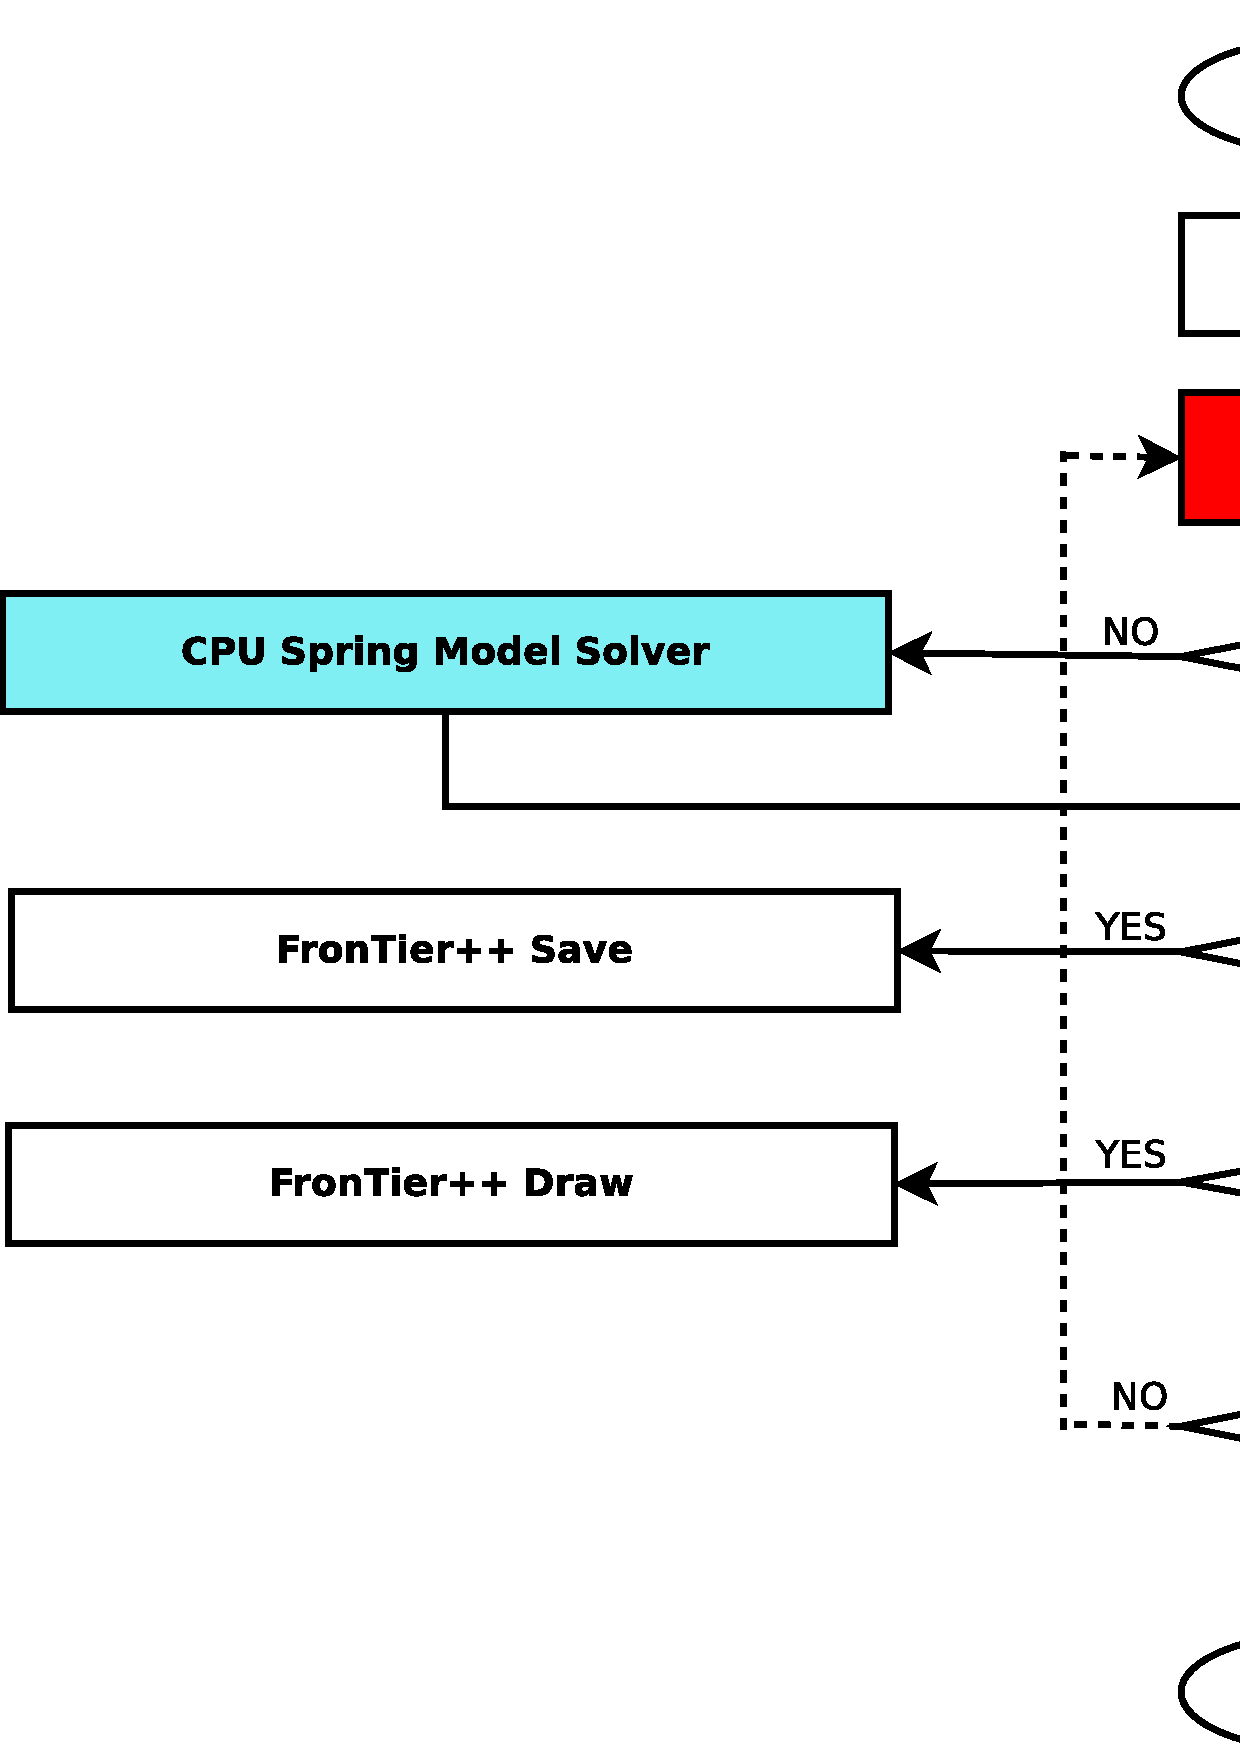
\includegraphics[width=1.0\textwidth]{figures/flowchart}
\caption{Flow chart of the complete simulation algorithm that involves
both fluid dynamics and elastic structure dynamics. The part inside the green
dash-dotted line is the work involves done by GPU.}
\label{fig:sm_flow_chart}
\end{figure}

Graphics Processing Unit (GPU) compution \cite{kirk2010programming} is to
use the GPUs together with CPUs to accelerate a general-pourpose scientific
and engineering application.
For the blue panel, we make use of the GPU technique to accelerate the
numerical calculation, i.e. the part inside the green dash-dotted line in
\Fig{sm_flow_chart}.
Solving the spring model by 4-th order Runge-Kutta method consists the
following steps:
\begin{enumerate}
\item Find the positions of all the neighbors of each spring vertex.
\item Calculate the total force on each spring vertex using Delingette method.\label{itm:2}
\item Calculate the acceleration of each vertex and update the location of
them.
\item Go to \ref{itm:2} if this is not the end of the Runge-Kutta; finish this
time step, otherwise.
\end{enumerate}
To accelerate the calculation of this part, we then shift it to the GPU
cores for massively parallel processing.
When we apply the GPU code to the complete parachute system, including both
the parachute canopy and all the suspension lines, we can achieve 16-21
$\times$ faster then pure CPU code for different types of parachutes, as
shown in \Tab{gpu_speedup}.
\begin{table*}
\centering
\begin{tabular}{cccccc}
\hline\hline
Parachute type & CPU/GPU & Time(s) & Avg time per step(s) & Speedup\\
\hline
\multirow{2}{*}{C-9} & CPU & 2805.85 & 3.39 & 1.00 \\
 & GPU & 131.90 & 0.16  & 21.2 \\
\hline
\multirow{2}{*}{G-11} & CPU & 5101.47 & 5.41 & 1.00 \\
 & GPU & 243.18 & 0.26 & 20.81 \\
\hline
\multirow{2}{*}{Intruder} & CPU & 1252.65 & 2.00 & 1.00 \\
 & GPU & 69.67 & 0.11 & 18.18 \\
\hline
\multirow{2}{*}{T-10} & CPU & 5540.02 & 5.99 & 1.00 \\
{} & GPU & 282.74 & 0.36 & 16.64\\
\hline
\multirow{2}{*}{T-11} & CPU & 6791.9 & 5.12 & 1.00 \\
{} & GPU & 352.07 & 0.29 & 17.66\\
\hline
\end{tabular}
\caption{A comparison of computational time between different parachute
types using CPU and GPU code. The speedup is calculated based on the
computing time by CPU.}
\label{tab:gpu_speedup}
\end{table*}

The solution for the red panel is to use multiple CPU cores; each CPU is in
charge of the calculation of one part of the computational domain.
The fluid computational domain is partitioned according to the computational
mesh grid, however, it is not the case for the canopy surface.
Intuitively, cutting the canopy surface through its edges is not reasonable
in the spring-mass model.
Therefore, a modified partitioning algorithm is applied which cut the canopy
surface according to the particles on it, as demonstrated in
\Fig{cpu_parallel} with $2 \times 2$ partitioning.
\begin{figure}[!ht]
\centering
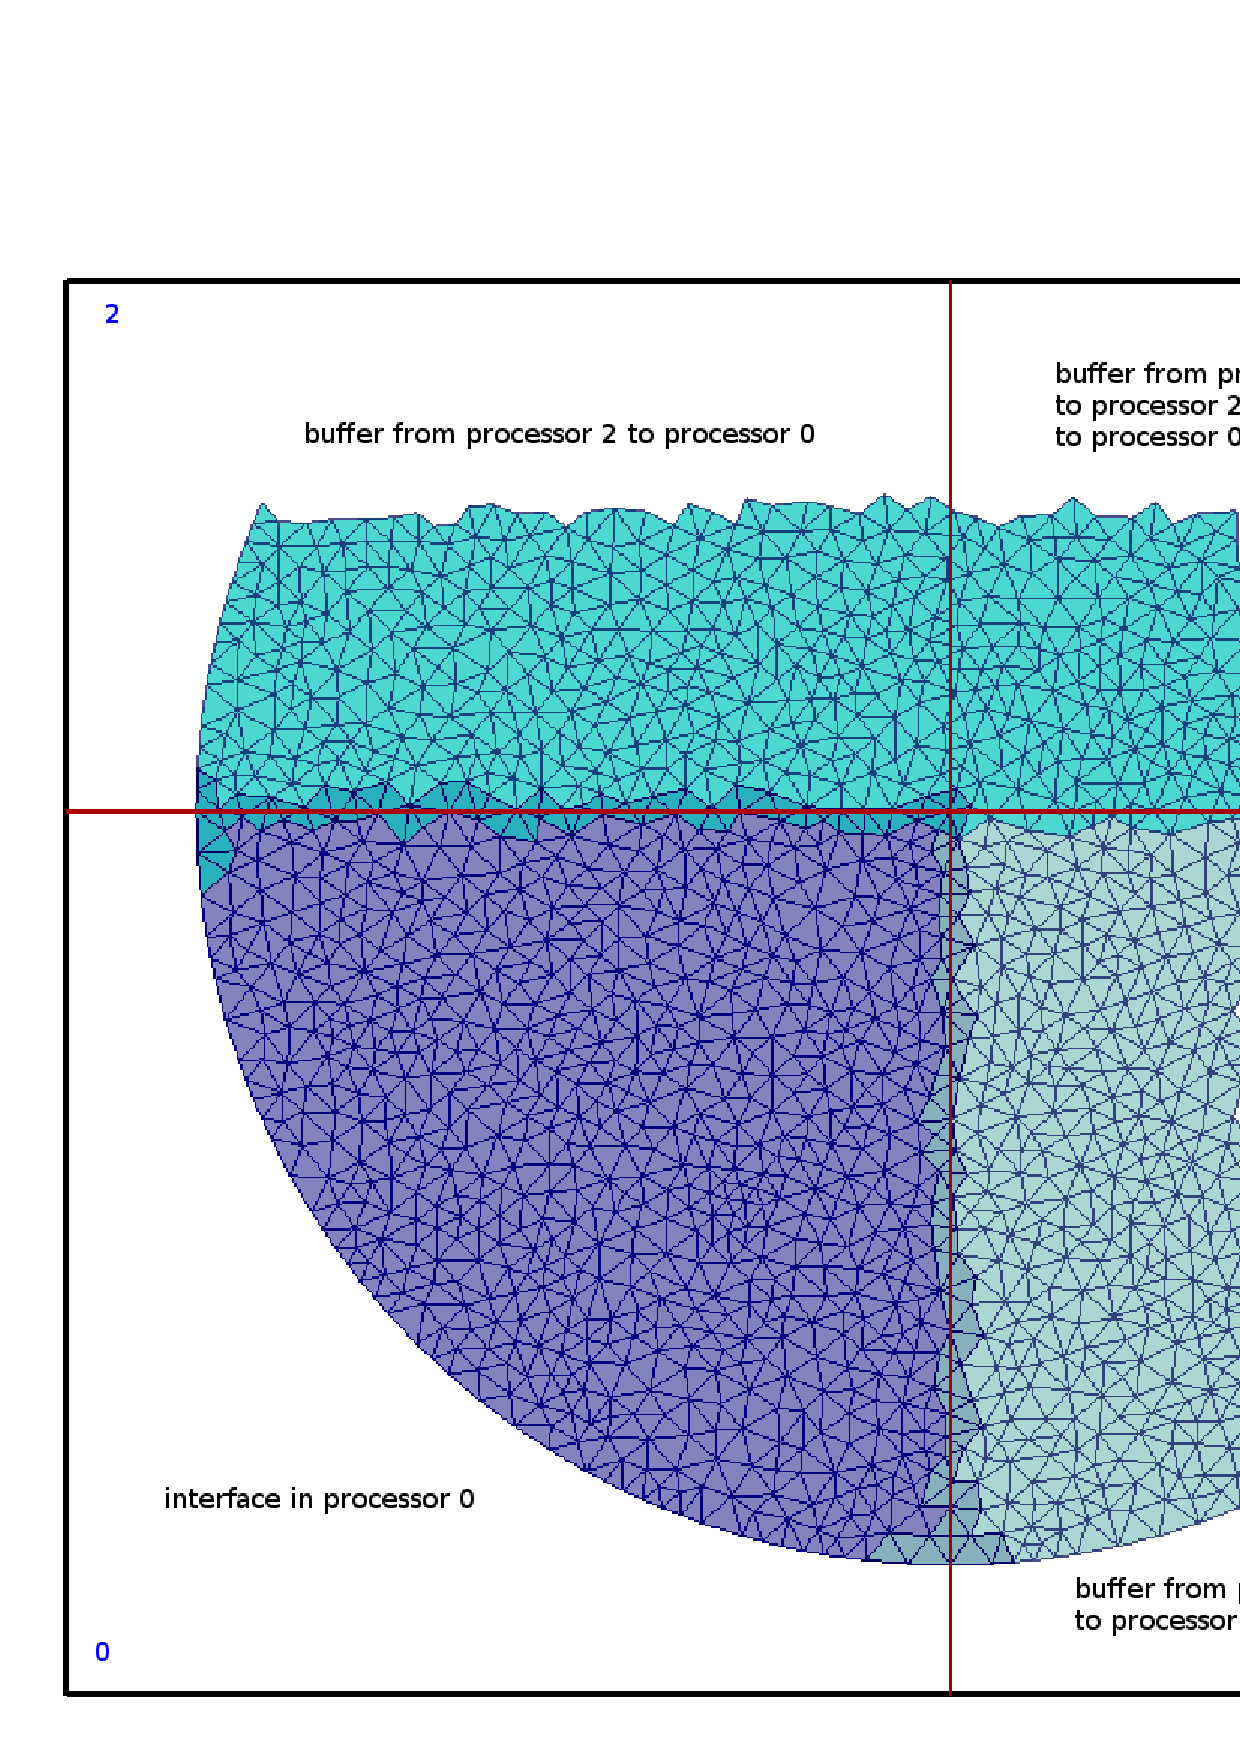
\includegraphics[width=0.66\textwidth]{figures/cpu_parallel}
\caption{A demonstration of the clipped interface in processors 0 and its
buffer interfaces from neighbor processors.}
\label{fig:cpu_parallel}
\end{figure}

The lower left part is the interface in processor 0, it received buffer
interface from two neighbor processors, 1 (lower right) and 2 (upper left).
The buffer interface provides neighbors to spring vertices that are close
to the sub-domain boundary.
Since the communication of buffer interface is done dimension by dimension,
the buffer interface from processor 2 contains part of the buffer interface
from processor 3 to processor 2.
With this partitioning algorithm, the spring-mass model work well with
multiple processors.

Furthermore, two techniques can be coupled together in the simulation of
parachute system.
\begin{enumerate}
\item Collect mass point information of the fabric structure from each
processor to the main processor.
\item Call the GPU-based spring model solver in the main processor.
\item Distrubute the updated information of each mass point to its
corresponding processor.
\end{enumerate}



\newpage
